% Created by tikzDevice version 0.12.3.1 on 2021-04-19 13:43:34
% !TEX encoding = UTF-8 Unicode
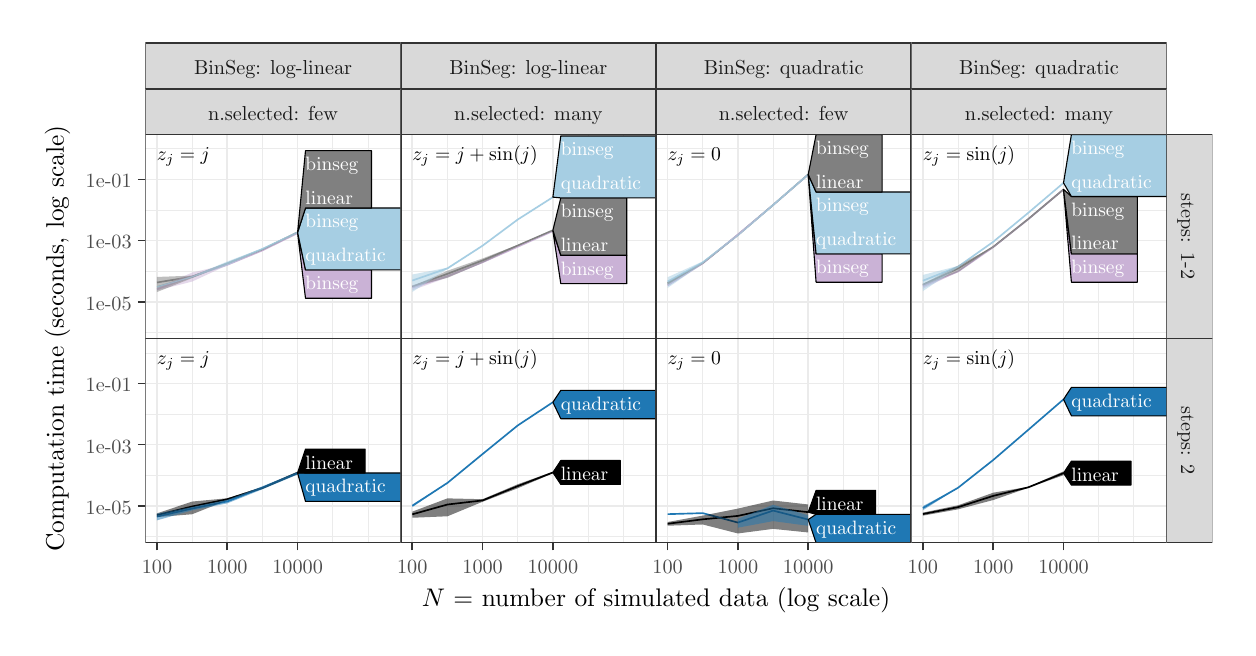
\begin{tikzpicture}[x=1pt,y=1pt]
\definecolor{fillColor}{RGB}{255,255,255}
\path[use as bounding box,fill=fillColor,fill opacity=0.00] (0,0) rectangle (433.62,216.81);
\begin{scope}
\path[clip] (  0.00,  0.00) rectangle (433.62,216.81);
\definecolor{drawColor}{RGB}{255,255,255}
\definecolor{fillColor}{RGB}{255,255,255}

\path[draw=drawColor,line width= 0.6pt,line join=round,line cap=round,fill=fillColor] (  0.00,  0.00) rectangle (433.62,216.81);
\end{scope}
\begin{scope}
\path[clip] ( 42.54,104.43) rectangle (134.79,178.17);
\definecolor{fillColor}{RGB}{255,255,255}

\path[fill=fillColor] ( 42.54,104.43) rectangle (134.79,178.17);
\definecolor{drawColor}{gray}{0.92}

\path[draw=drawColor,line width= 0.3pt,line join=round] ( 42.54,106.74) --
	(134.79,106.74);

\path[draw=drawColor,line width= 0.3pt,line join=round] ( 42.54,128.84) --
	(134.79,128.84);

\path[draw=drawColor,line width= 0.3pt,line join=round] ( 42.54,150.93) --
	(134.79,150.93);

\path[draw=drawColor,line width= 0.3pt,line join=round] ( 42.54,173.03) --
	(134.79,173.03);

\path[draw=drawColor,line width= 0.3pt,line join=round] ( 59.43,104.43) --
	( 59.43,178.17);

\path[draw=drawColor,line width= 0.3pt,line join=round] ( 84.84,104.43) --
	( 84.84,178.17);

\path[draw=drawColor,line width= 0.3pt,line join=round] (110.24,104.43) --
	(110.24,178.17);

\path[draw=drawColor,line width= 0.3pt,line join=round] (122.95,104.43) --
	(122.95,178.17);

\path[draw=drawColor,line width= 0.6pt,line join=round] ( 42.54,117.79) --
	(134.79,117.79);

\path[draw=drawColor,line width= 0.6pt,line join=round] ( 42.54,139.88) --
	(134.79,139.88);

\path[draw=drawColor,line width= 0.6pt,line join=round] ( 42.54,161.98) --
	(134.79,161.98);

\path[draw=drawColor,line width= 0.6pt,line join=round] ( 46.73,104.43) --
	( 46.73,178.17);

\path[draw=drawColor,line width= 0.6pt,line join=round] ( 72.14,104.43) --
	( 72.14,178.17);

\path[draw=drawColor,line width= 0.6pt,line join=round] ( 97.54,104.43) --
	( 97.54,178.17);
\definecolor{drawColor}{RGB}{0,0,0}

\node[text=drawColor,anchor=base west,inner sep=0pt, outer sep=0pt, scale=  0.71] at ( 46.73,168.94) {$z_j = j$};
\definecolor{drawColor}{RGB}{202,178,214}

\path[draw=drawColor,line width= 0.6pt,line join=round] ( 46.73,122.30) --
	( 59.43,126.96) --
	( 72.14,131.12) --
	( 84.84,136.34) --
	( 97.54,142.57);
\definecolor{drawColor}{gray}{0.50}

\path[draw=drawColor,line width= 0.6pt,line join=round] ( 46.73,124.74) --
	( 59.43,126.79) --
	( 72.14,131.63) --
	( 84.84,136.68) --
	( 97.54,142.88);
\definecolor{drawColor}{RGB}{166,206,227}

\path[draw=drawColor,line width= 0.6pt,line join=round] ( 46.73,123.12) --
	( 59.43,126.78) --
	( 72.14,131.67) --
	( 84.84,136.85) --
	( 97.54,142.83);
\definecolor{fillColor}{RGB}{202,178,214}

\path[fill=fillColor,fill opacity=0.50] ( 46.73,122.71) --
	( 59.43,128.32) --
	( 72.14,131.27) --
	( 84.84,136.43) --
	( 97.54,142.65) --
	( 97.54,142.49) --
	( 84.84,136.23) --
	( 72.14,130.96) --
	( 59.43,125.06) --
	( 46.73,121.85) --
	cycle;

\path[] ( 46.73,122.71) --
	( 59.43,128.32) --
	( 72.14,131.27) --
	( 84.84,136.43) --
	( 97.54,142.65);

\path[] ( 97.54,142.49) --
	( 84.84,136.23) --
	( 72.14,130.96) --
	( 59.43,125.06) --
	( 46.73,121.85);
\definecolor{fillColor}{RGB}{127,127,127}

\path[fill=fillColor,fill opacity=0.50] ( 46.73,126.73) --
	( 59.43,127.21) --
	( 72.14,131.90) --
	( 84.84,136.82) --
	( 97.54,143.01) --
	( 97.54,142.74) --
	( 84.84,136.55) --
	( 72.14,131.35) --
	( 59.43,126.33) --
	( 46.73,121.28) --
	cycle;

\path[] ( 46.73,126.73) --
	( 59.43,127.21) --
	( 72.14,131.90) --
	( 84.84,136.82) --
	( 97.54,143.01);

\path[] ( 97.54,142.74) --
	( 84.84,136.55) --
	( 72.14,131.35) --
	( 59.43,126.33) --
	( 46.73,121.28);
\definecolor{fillColor}{RGB}{166,206,227}

\path[fill=fillColor,fill opacity=0.50] ( 46.73,123.28) --
	( 59.43,126.98) --
	( 72.14,132.34) --
	( 84.84,137.09) --
	( 97.54,142.89) --
	( 97.54,142.76) --
	( 84.84,136.59) --
	( 72.14,130.90) --
	( 59.43,126.58) --
	( 46.73,122.96) --
	cycle;

\path[] ( 46.73,123.28) --
	( 59.43,126.98) --
	( 72.14,132.34) --
	( 84.84,137.09) --
	( 97.54,142.89);

\path[] ( 97.54,142.76) --
	( 84.84,136.59) --
	( 72.14,130.90) --
	( 59.43,126.58) --
	( 46.73,122.96);
\end{scope}
\begin{scope}
\path[clip] ( 42.54,104.43) rectangle (134.79,178.17);
\definecolor{drawColor}{RGB}{0,0,0}
\definecolor{fillColor}{RGB}{202,178,214}

\path[draw=drawColor,line width= 0.4pt,line join=round,line cap=round,fill=fillColor] ( 97.54,142.57) --
	(100.39,129.29) --
	(124.24,129.29) --
	(124.24,119.03) --
	(100.39,119.03) --
	cycle;
\definecolor{fillColor}{RGB}{166,206,227}

\path[draw=drawColor,line width= 0.4pt,line join=round,line cap=round,fill=fillColor] ( 97.54,142.83) --
	(100.39,151.65) --
	(135.84,151.65) --
	(135.84,129.29) --
	(100.39,129.29) --
	cycle;
\definecolor{fillColor}{gray}{0.50}

\path[draw=drawColor,line width= 0.4pt,line join=round,line cap=round,fill=fillColor] ( 97.54,142.88) --
	(100.39,172.38) --
	(124.24,172.38) --
	(124.24,151.65) --
	(100.39,151.65) --
	cycle;
\definecolor{drawColor}{RGB}{255,255,255}

\node[text=drawColor,anchor=base west,inner sep=0pt, outer sep=0pt, scale=  0.70] at (100.39,122.08) {binseg};

\node[text=drawColor,anchor=base west,inner sep=0pt, outer sep=0pt, scale=  0.70] at (100.39,144.44) {binseg};

\node[text=drawColor,anchor=base west,inner sep=0pt, outer sep=0pt, scale=  0.70] at (100.39,132.35) {quadratic};

\node[text=drawColor,anchor=base west,inner sep=0pt, outer sep=0pt, scale=  0.70] at (100.39,165.17) {binseg};

\node[text=drawColor,anchor=base west,inner sep=0pt, outer sep=0pt, scale=  0.70] at (100.39,153.07) {linear};
\definecolor{drawColor}{gray}{0.20}

\path[draw=drawColor,line width= 0.6pt,line join=round,line cap=round] ( 42.54,104.43) rectangle (134.79,178.17);
\end{scope}
\begin{scope}
\path[clip] ( 42.54, 30.69) rectangle (134.79,104.43);
\definecolor{fillColor}{RGB}{255,255,255}

\path[fill=fillColor] ( 42.54, 30.69) rectangle (134.79,104.43);
\definecolor{drawColor}{gray}{0.92}

\path[draw=drawColor,line width= 0.3pt,line join=round] ( 42.54, 33.00) --
	(134.79, 33.00);

\path[draw=drawColor,line width= 0.3pt,line join=round] ( 42.54, 55.10) --
	(134.79, 55.10);

\path[draw=drawColor,line width= 0.3pt,line join=round] ( 42.54, 77.19) --
	(134.79, 77.19);

\path[draw=drawColor,line width= 0.3pt,line join=round] ( 42.54, 99.28) --
	(134.79, 99.28);

\path[draw=drawColor,line width= 0.3pt,line join=round] ( 59.43, 30.69) --
	( 59.43,104.43);

\path[draw=drawColor,line width= 0.3pt,line join=round] ( 84.84, 30.69) --
	( 84.84,104.43);

\path[draw=drawColor,line width= 0.3pt,line join=round] (110.24, 30.69) --
	(110.24,104.43);

\path[draw=drawColor,line width= 0.3pt,line join=round] (122.95, 30.69) --
	(122.95,104.43);

\path[draw=drawColor,line width= 0.6pt,line join=round] ( 42.54, 44.05) --
	(134.79, 44.05);

\path[draw=drawColor,line width= 0.6pt,line join=round] ( 42.54, 66.14) --
	(134.79, 66.14);

\path[draw=drawColor,line width= 0.6pt,line join=round] ( 42.54, 88.24) --
	(134.79, 88.24);

\path[draw=drawColor,line width= 0.6pt,line join=round] ( 46.73, 30.69) --
	( 46.73,104.43);

\path[draw=drawColor,line width= 0.6pt,line join=round] ( 72.14, 30.69) --
	( 72.14,104.43);

\path[draw=drawColor,line width= 0.6pt,line join=round] ( 97.54, 30.69) --
	( 97.54,104.43);
\definecolor{drawColor}{RGB}{0,0,0}

\node[text=drawColor,anchor=base west,inner sep=0pt, outer sep=0pt, scale=  0.71] at ( 46.73, 95.20) {$z_j = j$};

\path[draw=drawColor,line width= 0.6pt,line join=round] ( 46.73, 40.67) --
	( 59.43, 43.80) --
	( 72.14, 46.41) --
	( 84.84, 50.50) --
	( 97.54, 55.96);
\definecolor{drawColor}{RGB}{31,120,180}

\path[draw=drawColor,line width= 0.6pt,line join=round] ( 46.73, 40.16) --
	( 59.43, 43.05) --
	( 72.14, 45.62) --
	( 84.84, 50.59) --
	( 97.54, 55.83);
\definecolor{fillColor}{RGB}{0,0,0}

\path[fill=fillColor,fill opacity=0.50] ( 46.73, 41.29) --
	( 59.43, 45.57) --
	( 72.14, 46.76) --
	( 84.84, 50.84) --
	( 97.54, 56.41) --
	( 97.54, 55.47) --
	( 84.84, 50.14) --
	( 72.14, 46.03) --
	( 59.43, 40.99) --
	( 46.73, 39.96) --
	cycle;

\path[] ( 46.73, 41.29) --
	( 59.43, 45.57) --
	( 72.14, 46.76) --
	( 84.84, 50.84) --
	( 97.54, 56.41);

\path[] ( 97.54, 55.47) --
	( 84.84, 50.14) --
	( 72.14, 46.03) --
	( 59.43, 40.99) --
	( 46.73, 39.96);
\definecolor{fillColor}{RGB}{31,120,180}

\path[fill=fillColor,fill opacity=0.50] ( 46.73, 41.22) --
	( 59.43, 43.63) --
	( 72.14, 46.22) --
	( 84.84, 51.10) --
	( 97.54, 56.29) --
	( 97.54, 55.33) --
	( 84.84, 50.01) --
	( 72.14, 44.92) --
	( 59.43, 42.39) --
	( 46.73, 38.78) --
	cycle;

\path[] ( 46.73, 41.22) --
	( 59.43, 43.63) --
	( 72.14, 46.22) --
	( 84.84, 51.10) --
	( 97.54, 56.29);

\path[] ( 97.54, 55.33) --
	( 84.84, 50.01) --
	( 72.14, 44.92) --
	( 59.43, 42.39) --
	( 46.73, 38.78);
\end{scope}
\begin{scope}
\path[clip] ( 42.54, 30.69) rectangle (134.79,104.43);
\definecolor{drawColor}{RGB}{0,0,0}
\definecolor{fillColor}{RGB}{31,120,180}

\path[draw=drawColor,line width= 0.4pt,line join=round,line cap=round,fill=fillColor] ( 97.54, 55.83) --
	(100.39, 55.90) --
	(135.84, 55.90) --
	(135.84, 45.63) --
	(100.39, 45.63) --
	cycle;
\definecolor{fillColor}{RGB}{0,0,0}

\path[draw=drawColor,line width= 0.4pt,line join=round,line cap=round,fill=fillColor] ( 97.54, 55.96) --
	(100.39, 64.53) --
	(121.91, 64.53) --
	(121.91, 55.90) --
	(100.39, 55.90) --
	cycle;
\definecolor{drawColor}{RGB}{255,255,255}

\node[text=drawColor,anchor=base west,inner sep=0pt, outer sep=0pt, scale=  0.70] at (100.39, 48.69) {quadratic};

\node[text=drawColor,anchor=base west,inner sep=0pt, outer sep=0pt, scale=  0.70] at (100.39, 57.32) {linear};
\definecolor{drawColor}{gray}{0.20}

\path[draw=drawColor,line width= 0.6pt,line join=round,line cap=round] ( 42.54, 30.69) rectangle (134.79,104.43);
\end{scope}
\begin{scope}
\path[clip] (134.79,104.43) rectangle (227.04,178.17);
\definecolor{fillColor}{RGB}{255,255,255}

\path[fill=fillColor] (134.79,104.43) rectangle (227.04,178.17);
\definecolor{drawColor}{gray}{0.92}

\path[draw=drawColor,line width= 0.3pt,line join=round] (134.79,106.74) --
	(227.04,106.74);

\path[draw=drawColor,line width= 0.3pt,line join=round] (134.79,128.84) --
	(227.04,128.84);

\path[draw=drawColor,line width= 0.3pt,line join=round] (134.79,150.93) --
	(227.04,150.93);

\path[draw=drawColor,line width= 0.3pt,line join=round] (134.79,173.03) --
	(227.04,173.03);

\path[draw=drawColor,line width= 0.3pt,line join=round] (151.69,104.43) --
	(151.69,178.17);

\path[draw=drawColor,line width= 0.3pt,line join=round] (177.09,104.43) --
	(177.09,178.17);

\path[draw=drawColor,line width= 0.3pt,line join=round] (202.50,104.43) --
	(202.50,178.17);

\path[draw=drawColor,line width= 0.3pt,line join=round] (215.20,104.43) --
	(215.20,178.17);

\path[draw=drawColor,line width= 0.6pt,line join=round] (134.79,117.79) --
	(227.04,117.79);

\path[draw=drawColor,line width= 0.6pt,line join=round] (134.79,139.88) --
	(227.04,139.88);

\path[draw=drawColor,line width= 0.6pt,line join=round] (134.79,161.98) --
	(227.04,161.98);

\path[draw=drawColor,line width= 0.6pt,line join=round] (138.98,104.43) --
	(138.98,178.17);

\path[draw=drawColor,line width= 0.6pt,line join=round] (164.39,104.43) --
	(164.39,178.17);

\path[draw=drawColor,line width= 0.6pt,line join=round] (189.79,104.43) --
	(189.79,178.17);
\definecolor{drawColor}{RGB}{0,0,0}

\node[text=drawColor,anchor=base west,inner sep=0pt, outer sep=0pt, scale=  0.71] at (138.98,168.94) {$z_j = j+\sin(j)$};
\definecolor{drawColor}{RGB}{202,178,214}

\path[draw=drawColor,line width= 0.6pt,line join=round] (138.98,122.90) --
	(151.69,126.98) --
	(164.39,132.05) --
	(177.09,137.66) --
	(189.79,143.32);
\definecolor{drawColor}{gray}{0.50}

\path[draw=drawColor,line width= 0.6pt,line join=round] (138.98,123.27) --
	(151.69,127.86) --
	(164.39,132.70) --
	(177.09,138.08) --
	(189.79,143.60);
\definecolor{drawColor}{RGB}{166,206,227}

\path[draw=drawColor,line width= 0.6pt,line join=round] (138.98,125.43) --
	(151.69,129.84) --
	(164.39,138.04) --
	(177.09,147.48) --
	(189.79,155.57);
\definecolor{fillColor}{RGB}{202,178,214}

\path[fill=fillColor,fill opacity=0.50] (138.98,123.70) --
	(151.69,127.39) --
	(164.39,132.19) --
	(177.09,137.83) --
	(189.79,143.36) --
	(189.79,143.28) --
	(177.09,137.49) --
	(164.39,131.91) --
	(151.69,126.53) --
	(138.98,121.93) --
	cycle;

\path[] (138.98,123.70) --
	(151.69,127.39) --
	(164.39,132.19) --
	(177.09,137.83) --
	(189.79,143.36);

\path[] (189.79,143.28) --
	(177.09,137.49) --
	(164.39,131.91) --
	(151.69,126.53) --
	(138.98,121.93);
\definecolor{fillColor}{RGB}{127,127,127}

\path[fill=fillColor,fill opacity=0.50] (138.98,123.36) --
	(151.69,128.98) --
	(164.39,133.42) --
	(177.09,138.33) --
	(189.79,143.67) --
	(189.79,143.52) --
	(177.09,137.82) --
	(164.39,131.85) --
	(151.69,126.41) --
	(138.98,123.18) --
	cycle;

\path[] (138.98,123.36) --
	(151.69,128.98) --
	(164.39,133.42) --
	(177.09,138.33) --
	(189.79,143.67);

\path[] (189.79,143.52) --
	(177.09,137.82) --
	(164.39,131.85) --
	(151.69,126.41) --
	(138.98,123.18);
\definecolor{fillColor}{RGB}{166,206,227}

\path[fill=fillColor,fill opacity=0.50] (138.98,127.61) --
	(151.69,130.08) --
	(164.39,138.06) --
	(177.09,147.50) --
	(189.79,155.59) --
	(189.79,155.55) --
	(177.09,147.46) --
	(164.39,138.01) --
	(151.69,129.59) --
	(138.98,121.31) --
	cycle;

\path[] (138.98,127.61) --
	(151.69,130.08) --
	(164.39,138.06) --
	(177.09,147.50) --
	(189.79,155.59);

\path[] (189.79,155.55) --
	(177.09,147.46) --
	(164.39,138.01) --
	(151.69,129.59) --
	(138.98,121.31);
\end{scope}
\begin{scope}
\path[clip] (134.79,104.43) rectangle (227.04,178.17);
\definecolor{drawColor}{RGB}{0,0,0}
\definecolor{fillColor}{RGB}{202,178,214}

\path[draw=drawColor,line width= 0.4pt,line join=round,line cap=round,fill=fillColor] (189.79,143.32) --
	(192.64,134.57) --
	(216.49,134.57) --
	(216.49,124.31) --
	(192.64,124.31) --
	cycle;
\definecolor{fillColor}{gray}{0.50}

\path[draw=drawColor,line width= 0.4pt,line join=round,line cap=round,fill=fillColor] (189.79,143.60) --
	(192.64,155.30) --
	(216.49,155.30) --
	(216.49,134.57) --
	(192.64,134.57) --
	cycle;
\definecolor{fillColor}{RGB}{166,206,227}

\path[draw=drawColor,line width= 0.4pt,line join=round,line cap=round,fill=fillColor] (189.79,155.57) --
	(192.64,177.66) --
	(228.10,177.66) --
	(228.10,155.30) --
	(192.64,155.30) --
	cycle;
\definecolor{drawColor}{RGB}{255,255,255}

\node[text=drawColor,anchor=base west,inner sep=0pt, outer sep=0pt, scale=  0.70] at (192.64,127.36) {binseg};

\node[text=drawColor,anchor=base west,inner sep=0pt, outer sep=0pt, scale=  0.70] at (192.64,148.09) {binseg};

\node[text=drawColor,anchor=base west,inner sep=0pt, outer sep=0pt, scale=  0.70] at (192.64,136.00) {linear};

\node[text=drawColor,anchor=base west,inner sep=0pt, outer sep=0pt, scale=  0.70] at (192.64,170.45) {binseg};

\node[text=drawColor,anchor=base west,inner sep=0pt, outer sep=0pt, scale=  0.70] at (192.64,158.35) {quadratic};
\definecolor{drawColor}{gray}{0.20}

\path[draw=drawColor,line width= 0.6pt,line join=round,line cap=round] (134.79,104.43) rectangle (227.04,178.17);
\end{scope}
\begin{scope}
\path[clip] (134.79, 30.69) rectangle (227.04,104.43);
\definecolor{fillColor}{RGB}{255,255,255}

\path[fill=fillColor] (134.79, 30.69) rectangle (227.04,104.43);
\definecolor{drawColor}{gray}{0.92}

\path[draw=drawColor,line width= 0.3pt,line join=round] (134.79, 33.00) --
	(227.04, 33.00);

\path[draw=drawColor,line width= 0.3pt,line join=round] (134.79, 55.10) --
	(227.04, 55.10);

\path[draw=drawColor,line width= 0.3pt,line join=round] (134.79, 77.19) --
	(227.04, 77.19);

\path[draw=drawColor,line width= 0.3pt,line join=round] (134.79, 99.28) --
	(227.04, 99.28);

\path[draw=drawColor,line width= 0.3pt,line join=round] (151.69, 30.69) --
	(151.69,104.43);

\path[draw=drawColor,line width= 0.3pt,line join=round] (177.09, 30.69) --
	(177.09,104.43);

\path[draw=drawColor,line width= 0.3pt,line join=round] (202.50, 30.69) --
	(202.50,104.43);

\path[draw=drawColor,line width= 0.3pt,line join=round] (215.20, 30.69) --
	(215.20,104.43);

\path[draw=drawColor,line width= 0.6pt,line join=round] (134.79, 44.05) --
	(227.04, 44.05);

\path[draw=drawColor,line width= 0.6pt,line join=round] (134.79, 66.14) --
	(227.04, 66.14);

\path[draw=drawColor,line width= 0.6pt,line join=round] (134.79, 88.24) --
	(227.04, 88.24);

\path[draw=drawColor,line width= 0.6pt,line join=round] (138.98, 30.69) --
	(138.98,104.43);

\path[draw=drawColor,line width= 0.6pt,line join=round] (164.39, 30.69) --
	(164.39,104.43);

\path[draw=drawColor,line width= 0.6pt,line join=round] (189.79, 30.69) --
	(189.79,104.43);
\definecolor{drawColor}{RGB}{0,0,0}

\node[text=drawColor,anchor=base west,inner sep=0pt, outer sep=0pt, scale=  0.71] at (138.98, 95.20) {$z_j = j+\sin(j)$};

\path[draw=drawColor,line width= 0.6pt,line join=round] (138.98, 40.95) --
	(151.69, 44.50) --
	(164.39, 45.98) --
	(177.09, 51.16) --
	(189.79, 56.08);
\definecolor{drawColor}{RGB}{31,120,180}

\path[draw=drawColor,line width= 0.6pt,line join=round] (138.98, 44.04) --
	(151.69, 52.32) --
	(164.39, 62.75) --
	(177.09, 73.08) --
	(189.79, 81.46);
\definecolor{fillColor}{RGB}{0,0,0}

\path[fill=fillColor,fill opacity=0.50] (138.98, 41.93) --
	(151.69, 46.72) --
	(164.39, 46.42) --
	(177.09, 51.82) --
	(189.79, 56.34) --
	(189.79, 55.80) --
	(177.09, 50.38) --
	(164.39, 45.50) --
	(151.69, 40.25) --
	(138.98, 39.72) --
	cycle;

\path[] (138.98, 41.93) --
	(151.69, 46.72) --
	(164.39, 46.42) --
	(177.09, 51.82) --
	(189.79, 56.34);

\path[] (189.79, 55.80) --
	(177.09, 50.38) --
	(164.39, 45.50) --
	(151.69, 40.25) --
	(138.98, 39.72);
\definecolor{fillColor}{RGB}{31,120,180}

\path[fill=fillColor,fill opacity=0.50] (138.98, 44.47) --
	(151.69, 52.42) --
	(164.39, 62.86) --
	(177.09, 73.10) --
	(189.79, 81.47) --
	(189.79, 81.44) --
	(177.09, 73.07) --
	(164.39, 62.63) --
	(151.69, 52.21) --
	(138.98, 43.57) --
	cycle;

\path[] (138.98, 44.47) --
	(151.69, 52.42) --
	(164.39, 62.86) --
	(177.09, 73.10) --
	(189.79, 81.47);

\path[] (189.79, 81.44) --
	(177.09, 73.07) --
	(164.39, 62.63) --
	(151.69, 52.21) --
	(138.98, 43.57);
\end{scope}
\begin{scope}
\path[clip] (134.79, 30.69) rectangle (227.04,104.43);
\definecolor{drawColor}{RGB}{0,0,0}
\definecolor{fillColor}{RGB}{0,0,0}

\path[draw=drawColor,line width= 0.4pt,line join=round,line cap=round,fill=fillColor] (189.79, 56.08) --
	(192.64, 60.39) --
	(214.16, 60.39) --
	(214.16, 51.76) --
	(192.64, 51.76) --
	cycle;
\definecolor{fillColor}{RGB}{31,120,180}

\path[draw=drawColor,line width= 0.4pt,line join=round,line cap=round,fill=fillColor] (189.79, 81.46) --
	(192.64, 85.77) --
	(228.10, 85.77) --
	(228.10, 75.51) --
	(192.64, 75.51) --
	cycle;
\definecolor{drawColor}{RGB}{255,255,255}

\node[text=drawColor,anchor=base west,inner sep=0pt, outer sep=0pt, scale=  0.70] at (192.64, 53.19) {linear};

\node[text=drawColor,anchor=base west,inner sep=0pt, outer sep=0pt, scale=  0.70] at (192.64, 78.56) {quadratic};
\definecolor{drawColor}{gray}{0.20}

\path[draw=drawColor,line width= 0.6pt,line join=round,line cap=round] (134.79, 30.69) rectangle (227.04,104.43);
\end{scope}
\begin{scope}
\path[clip] (227.04,104.43) rectangle (319.30,178.17);
\definecolor{fillColor}{RGB}{255,255,255}

\path[fill=fillColor] (227.04,104.43) rectangle (319.30,178.17);
\definecolor{drawColor}{gray}{0.92}

\path[draw=drawColor,line width= 0.3pt,line join=round] (227.04,106.74) --
	(319.30,106.74);

\path[draw=drawColor,line width= 0.3pt,line join=round] (227.04,128.84) --
	(319.30,128.84);

\path[draw=drawColor,line width= 0.3pt,line join=round] (227.04,150.93) --
	(319.30,150.93);

\path[draw=drawColor,line width= 0.3pt,line join=round] (227.04,173.03) --
	(319.30,173.03);

\path[draw=drawColor,line width= 0.3pt,line join=round] (243.94,104.43) --
	(243.94,178.17);

\path[draw=drawColor,line width= 0.3pt,line join=round] (269.35,104.43) --
	(269.35,178.17);

\path[draw=drawColor,line width= 0.3pt,line join=round] (294.75,104.43) --
	(294.75,178.17);

\path[draw=drawColor,line width= 0.3pt,line join=round] (307.45,104.43) --
	(307.45,178.17);

\path[draw=drawColor,line width= 0.6pt,line join=round] (227.04,117.79) --
	(319.30,117.79);

\path[draw=drawColor,line width= 0.6pt,line join=round] (227.04,139.88) --
	(319.30,139.88);

\path[draw=drawColor,line width= 0.6pt,line join=round] (227.04,161.98) --
	(319.30,161.98);

\path[draw=drawColor,line width= 0.6pt,line join=round] (231.24,104.43) --
	(231.24,178.17);

\path[draw=drawColor,line width= 0.6pt,line join=round] (256.64,104.43) --
	(256.64,178.17);

\path[draw=drawColor,line width= 0.6pt,line join=round] (282.05,104.43) --
	(282.05,178.17);
\definecolor{drawColor}{RGB}{0,0,0}

\node[text=drawColor,anchor=base west,inner sep=0pt, outer sep=0pt, scale=  0.71] at (231.24,168.94) {$z_j = 0$};
\definecolor{drawColor}{RGB}{202,178,214}

\path[draw=drawColor,line width= 0.6pt,line join=round] (231.24,123.68) --
	(243.94,131.63) --
	(256.64,142.06) --
	(269.35,152.73) --
	(282.05,163.71);
\definecolor{drawColor}{gray}{0.50}

\path[draw=drawColor,line width= 0.6pt,line join=round] (231.24,124.42) --
	(243.94,131.80) --
	(256.64,141.87) --
	(269.35,152.72) --
	(282.05,163.77);
\definecolor{drawColor}{RGB}{166,206,227}

\path[draw=drawColor,line width= 0.6pt,line join=round] (231.24,125.07) --
	(243.94,131.96) --
	(256.64,141.85) --
	(269.35,152.73) --
	(282.05,163.76);
\definecolor{fillColor}{RGB}{202,178,214}

\path[fill=fillColor,fill opacity=0.50] (231.24,123.82) --
	(243.94,131.69) --
	(256.64,142.41) --
	(269.35,152.74) --
	(282.05,163.74) --
	(282.05,163.69) --
	(269.35,152.71) --
	(256.64,141.67) --
	(243.94,131.57) --
	(231.24,123.55) --
	cycle;

\path[] (231.24,123.82) --
	(243.94,131.69) --
	(256.64,142.41) --
	(269.35,152.74) --
	(282.05,163.74);

\path[] (282.05,163.69) --
	(269.35,152.71) --
	(256.64,141.67) --
	(243.94,131.57) --
	(231.24,123.55);
\definecolor{fillColor}{RGB}{127,127,127}

\path[fill=fillColor,fill opacity=0.50] (231.24,124.87) --
	(243.94,131.97) --
	(256.64,141.89) --
	(269.35,152.73) --
	(282.05,163.86) --
	(282.05,163.68) --
	(269.35,152.71) --
	(256.64,141.85) --
	(243.94,131.62) --
	(231.24,123.92) --
	cycle;

\path[] (231.24,124.87) --
	(243.94,131.97) --
	(256.64,141.89) --
	(269.35,152.73) --
	(282.05,163.86);

\path[] (282.05,163.68) --
	(269.35,152.71) --
	(256.64,141.85) --
	(243.94,131.62) --
	(231.24,123.92);
\definecolor{fillColor}{RGB}{166,206,227}

\path[fill=fillColor,fill opacity=0.50] (231.24,126.63) --
	(243.94,132.36) --
	(256.64,141.88) --
	(269.35,152.75) --
	(282.05,163.89) --
	(282.05,163.63) --
	(269.35,152.71) --
	(256.64,141.83) --
	(243.94,131.52) --
	(231.24,122.76) --
	cycle;

\path[] (231.24,126.63) --
	(243.94,132.36) --
	(256.64,141.88) --
	(269.35,152.75) --
	(282.05,163.89);

\path[] (282.05,163.63) --
	(269.35,152.71) --
	(256.64,141.83) --
	(243.94,131.52) --
	(231.24,122.76);
\end{scope}
\begin{scope}
\path[clip] (227.04,104.43) rectangle (319.30,178.17);
\definecolor{drawColor}{RGB}{0,0,0}
\definecolor{fillColor}{RGB}{202,178,214}

\path[draw=drawColor,line width= 0.4pt,line join=round,line cap=round,fill=fillColor] (282.05,163.71) --
	(284.89,135.08) --
	(308.75,135.08) --
	(308.75,124.82) --
	(284.89,124.82) --
	cycle;
\definecolor{fillColor}{RGB}{166,206,227}

\path[draw=drawColor,line width= 0.4pt,line join=round,line cap=round,fill=fillColor] (282.05,163.76) --
	(284.89,157.44) --
	(320.35,157.44) --
	(320.35,135.08) --
	(284.89,135.08) --
	cycle;
\definecolor{fillColor}{gray}{0.50}

\path[draw=drawColor,line width= 0.4pt,line join=round,line cap=round,fill=fillColor] (282.05,163.77) --
	(284.89,178.17) --
	(308.75,178.17) --
	(308.75,157.44) --
	(284.89,157.44) --
	cycle;
\definecolor{drawColor}{RGB}{255,255,255}

\node[text=drawColor,anchor=base west,inner sep=0pt, outer sep=0pt, scale=  0.70] at (284.89,127.87) {binseg};

\node[text=drawColor,anchor=base west,inner sep=0pt, outer sep=0pt, scale=  0.70] at (284.89,150.23) {binseg};

\node[text=drawColor,anchor=base west,inner sep=0pt, outer sep=0pt, scale=  0.70] at (284.89,138.14) {quadratic};

\node[text=drawColor,anchor=base west,inner sep=0pt, outer sep=0pt, scale=  0.70] at (284.89,170.96) {binseg};

\node[text=drawColor,anchor=base west,inner sep=0pt, outer sep=0pt, scale=  0.70] at (284.89,158.86) {linear};
\definecolor{drawColor}{gray}{0.20}

\path[draw=drawColor,line width= 0.6pt,line join=round,line cap=round] (227.04,104.43) rectangle (319.30,178.17);
\end{scope}
\begin{scope}
\path[clip] (227.04, 30.69) rectangle (319.30,104.43);
\definecolor{fillColor}{RGB}{255,255,255}

\path[fill=fillColor] (227.04, 30.69) rectangle (319.30,104.43);
\definecolor{drawColor}{gray}{0.92}

\path[draw=drawColor,line width= 0.3pt,line join=round] (227.04, 33.00) --
	(319.30, 33.00);

\path[draw=drawColor,line width= 0.3pt,line join=round] (227.04, 55.10) --
	(319.30, 55.10);

\path[draw=drawColor,line width= 0.3pt,line join=round] (227.04, 77.19) --
	(319.30, 77.19);

\path[draw=drawColor,line width= 0.3pt,line join=round] (227.04, 99.28) --
	(319.30, 99.28);

\path[draw=drawColor,line width= 0.3pt,line join=round] (243.94, 30.69) --
	(243.94,104.43);

\path[draw=drawColor,line width= 0.3pt,line join=round] (269.35, 30.69) --
	(269.35,104.43);

\path[draw=drawColor,line width= 0.3pt,line join=round] (294.75, 30.69) --
	(294.75,104.43);

\path[draw=drawColor,line width= 0.3pt,line join=round] (307.45, 30.69) --
	(307.45,104.43);

\path[draw=drawColor,line width= 0.6pt,line join=round] (227.04, 44.05) --
	(319.30, 44.05);

\path[draw=drawColor,line width= 0.6pt,line join=round] (227.04, 66.14) --
	(319.30, 66.14);

\path[draw=drawColor,line width= 0.6pt,line join=round] (227.04, 88.24) --
	(319.30, 88.24);

\path[draw=drawColor,line width= 0.6pt,line join=round] (231.24, 30.69) --
	(231.24,104.43);

\path[draw=drawColor,line width= 0.6pt,line join=round] (256.64, 30.69) --
	(256.64,104.43);

\path[draw=drawColor,line width= 0.6pt,line join=round] (282.05, 30.69) --
	(282.05,104.43);
\definecolor{drawColor}{RGB}{0,0,0}

\node[text=drawColor,anchor=base west,inner sep=0pt, outer sep=0pt, scale=  0.71] at (231.24, 95.20) {$z_j = 0$};

\path[draw=drawColor,line width= 0.6pt,line join=round] (231.24, 37.55) --
	(243.94, 39.15) --
	(256.64, 40.39) --
	(269.35, 43.16) --
	(282.05, 41.74);
\definecolor{drawColor}{RGB}{31,120,180}

\path[draw=drawColor,line width= 0.6pt,line join=round] (231.24, 41.02) --
	(243.94, 41.39) --
	(256.64, 37.98) --
	(269.35, 42.31) --
	(282.05, 39.07);
\definecolor{fillColor}{RGB}{0,0,0}

\path[fill=fillColor,fill opacity=0.50] (231.24, 38.17) --
	(243.94, 40.49) --
	(256.64, 43.03) --
	(269.35, 45.95) --
	(282.05, 44.52) --
	(282.05, 34.40) --
	(269.35, 35.70) --
	(256.64, 34.04) --
	(243.94, 37.29) --
	(231.24, 36.84) --
	cycle;

\path[] (231.24, 38.17) --
	(243.94, 40.49) --
	(256.64, 43.03) --
	(269.35, 45.95) --
	(282.05, 44.52);

\path[] (282.05, 34.40) --
	(269.35, 35.70) --
	(256.64, 34.04) --
	(243.94, 37.29) --
	(231.24, 36.84);
\definecolor{fillColor}{RGB}{31,120,180}

\path[fill=fillColor,fill opacity=0.50] (256.64, 39.31) --
	(269.35, 44.41) --
	(282.05, 40.60) --
	(282.05, 36.81) --
	(269.35, 38.51) --
	(256.64, 36.13) --
	cycle;

\path[] (256.64, 39.31) --
	(269.35, 44.41) --
	(282.05, 40.60);

\path[] (282.05, 36.81) --
	(269.35, 38.51) --
	(256.64, 36.13);
\end{scope}
\begin{scope}
\path[clip] (227.04, 30.69) rectangle (319.30,104.43);
\definecolor{drawColor}{RGB}{0,0,0}
\definecolor{fillColor}{RGB}{31,120,180}

\path[draw=drawColor,line width= 0.4pt,line join=round,line cap=round,fill=fillColor] (282.05, 39.07) --
	(284.89, 40.95) --
	(320.35, 40.95) --
	(320.35, 30.69) --
	(284.89, 30.69) --
	cycle;
\definecolor{fillColor}{RGB}{0,0,0}

\path[draw=drawColor,line width= 0.4pt,line join=round,line cap=round,fill=fillColor] (282.05, 41.74) --
	(284.89, 49.58) --
	(306.42, 49.58) --
	(306.42, 40.95) --
	(284.89, 40.95) --
	cycle;
\definecolor{drawColor}{RGB}{255,255,255}

\node[text=drawColor,anchor=base west,inner sep=0pt, outer sep=0pt, scale=  0.70] at (284.89, 33.74) {quadratic};

\node[text=drawColor,anchor=base west,inner sep=0pt, outer sep=0pt, scale=  0.70] at (284.89, 42.37) {linear};
\definecolor{drawColor}{gray}{0.20}

\path[draw=drawColor,line width= 0.6pt,line join=round,line cap=round] (227.04, 30.69) rectangle (319.30,104.43);
\end{scope}
\begin{scope}
\path[clip] (319.30,104.43) rectangle (411.55,178.17);
\definecolor{fillColor}{RGB}{255,255,255}

\path[fill=fillColor] (319.30,104.43) rectangle (411.55,178.17);
\definecolor{drawColor}{gray}{0.92}

\path[draw=drawColor,line width= 0.3pt,line join=round] (319.30,106.74) --
	(411.55,106.74);

\path[draw=drawColor,line width= 0.3pt,line join=round] (319.30,128.84) --
	(411.55,128.84);

\path[draw=drawColor,line width= 0.3pt,line join=round] (319.30,150.93) --
	(411.55,150.93);

\path[draw=drawColor,line width= 0.3pt,line join=round] (319.30,173.03) --
	(411.55,173.03);

\path[draw=drawColor,line width= 0.3pt,line join=round] (336.19,104.43) --
	(336.19,178.17);

\path[draw=drawColor,line width= 0.3pt,line join=round] (361.60,104.43) --
	(361.60,178.17);

\path[draw=drawColor,line width= 0.3pt,line join=round] (387.00,104.43) --
	(387.00,178.17);

\path[draw=drawColor,line width= 0.3pt,line join=round] (399.71,104.43) --
	(399.71,178.17);

\path[draw=drawColor,line width= 0.6pt,line join=round] (319.30,117.79) --
	(411.55,117.79);

\path[draw=drawColor,line width= 0.6pt,line join=round] (319.30,139.88) --
	(411.55,139.88);

\path[draw=drawColor,line width= 0.6pt,line join=round] (319.30,161.98) --
	(411.55,161.98);

\path[draw=drawColor,line width= 0.6pt,line join=round] (323.49,104.43) --
	(323.49,178.17);

\path[draw=drawColor,line width= 0.6pt,line join=round] (348.90,104.43) --
	(348.90,178.17);

\path[draw=drawColor,line width= 0.6pt,line join=round] (374.30,104.43) --
	(374.30,178.17);
\definecolor{drawColor}{RGB}{0,0,0}

\node[text=drawColor,anchor=base west,inner sep=0pt, outer sep=0pt, scale=  0.71] at (323.49,168.94) {$z_j = \sin(j)$};
\definecolor{drawColor}{RGB}{202,178,214}

\path[draw=drawColor,line width= 0.6pt,line join=round] (323.49,123.37) --
	(336.19,128.72) --
	(348.90,137.51) --
	(361.60,147.63) --
	(374.30,158.36);
\definecolor{drawColor}{gray}{0.50}

\path[draw=drawColor,line width= 0.6pt,line join=round] (323.49,123.93) --
	(336.19,129.81) --
	(348.90,137.60) --
	(361.60,147.70) --
	(374.30,158.37);
\definecolor{drawColor}{RGB}{166,206,227}

\path[draw=drawColor,line width= 0.6pt,line join=round] (323.49,125.38) --
	(336.19,130.44) --
	(348.90,139.43) --
	(361.60,149.93) --
	(374.30,160.72);
\definecolor{fillColor}{RGB}{202,178,214}

\path[fill=fillColor,fill opacity=0.50] (323.49,124.13) --
	(336.19,128.86) --
	(348.90,137.63) --
	(361.60,147.66) --
	(374.30,158.44) --
	(374.30,158.29) --
	(361.60,147.61) --
	(348.90,137.39) --
	(336.19,128.58) --
	(323.49,122.48) --
	cycle;

\path[] (323.49,124.13) --
	(336.19,128.86) --
	(348.90,137.63) --
	(361.60,147.66) --
	(374.30,158.44);

\path[] (374.30,158.29) --
	(361.60,147.61) --
	(348.90,137.39) --
	(336.19,128.58) --
	(323.49,122.48);
\definecolor{fillColor}{RGB}{127,127,127}

\path[fill=fillColor,fill opacity=0.50] (323.49,124.22) --
	(336.19,130.83) --
	(348.90,137.65) --
	(361.60,147.72) --
	(374.30,158.38) --
	(374.30,158.35) --
	(361.60,147.67) --
	(348.90,137.55) --
	(336.19,128.51) --
	(323.49,123.62) --
	cycle;

\path[] (323.49,124.22) --
	(336.19,130.83) --
	(348.90,137.65) --
	(361.60,147.72) --
	(374.30,158.38);

\path[] (374.30,158.35) --
	(361.60,147.67) --
	(348.90,137.55) --
	(336.19,128.51) --
	(323.49,123.62);
\definecolor{fillColor}{RGB}{166,206,227}

\path[fill=fillColor,fill opacity=0.50] (323.49,127.46) --
	(336.19,130.71) --
	(348.90,139.47) --
	(361.60,149.97) --
	(374.30,160.73) --
	(374.30,160.71) --
	(361.60,149.88) --
	(348.90,139.40) --
	(336.19,130.15) --
	(323.49,121.62) --
	cycle;

\path[] (323.49,127.46) --
	(336.19,130.71) --
	(348.90,139.47) --
	(361.60,149.97) --
	(374.30,160.73);

\path[] (374.30,160.71) --
	(361.60,149.88) --
	(348.90,139.40) --
	(336.19,130.15) --
	(323.49,121.62);
\end{scope}
\begin{scope}
\path[clip] (319.30,104.43) rectangle (411.55,178.17);
\definecolor{drawColor}{RGB}{0,0,0}
\definecolor{fillColor}{RGB}{202,178,214}

\path[draw=drawColor,line width= 0.4pt,line join=round,line cap=round,fill=fillColor] (374.30,158.36) --
	(377.15,135.08) --
	(401.00,135.08) --
	(401.00,124.82) --
	(377.15,124.82) --
	cycle;
\definecolor{fillColor}{gray}{0.50}

\path[draw=drawColor,line width= 0.4pt,line join=round,line cap=round,fill=fillColor] (374.30,158.37) --
	(377.15,155.81) --
	(401.00,155.81) --
	(401.00,135.08) --
	(377.15,135.08) --
	cycle;
\definecolor{fillColor}{RGB}{166,206,227}

\path[draw=drawColor,line width= 0.4pt,line join=round,line cap=round,fill=fillColor] (374.30,160.72) --
	(377.15,178.17) --
	(412.60,178.17) --
	(412.60,155.81) --
	(377.15,155.81) --
	cycle;
\definecolor{drawColor}{RGB}{255,255,255}

\node[text=drawColor,anchor=base west,inner sep=0pt, outer sep=0pt, scale=  0.70] at (377.15,127.87) {binseg};

\node[text=drawColor,anchor=base west,inner sep=0pt, outer sep=0pt, scale=  0.70] at (377.15,148.60) {binseg};

\node[text=drawColor,anchor=base west,inner sep=0pt, outer sep=0pt, scale=  0.70] at (377.15,136.50) {linear};

\node[text=drawColor,anchor=base west,inner sep=0pt, outer sep=0pt, scale=  0.70] at (377.15,170.96) {binseg};

\node[text=drawColor,anchor=base west,inner sep=0pt, outer sep=0pt, scale=  0.70] at (377.15,158.86) {quadratic};
\definecolor{drawColor}{gray}{0.20}

\path[draw=drawColor,line width= 0.6pt,line join=round,line cap=round] (319.30,104.43) rectangle (411.55,178.17);
\end{scope}
\begin{scope}
\path[clip] (319.30, 30.69) rectangle (411.55,104.43);
\definecolor{fillColor}{RGB}{255,255,255}

\path[fill=fillColor] (319.30, 30.69) rectangle (411.55,104.43);
\definecolor{drawColor}{gray}{0.92}

\path[draw=drawColor,line width= 0.3pt,line join=round] (319.30, 33.00) --
	(411.55, 33.00);

\path[draw=drawColor,line width= 0.3pt,line join=round] (319.30, 55.10) --
	(411.55, 55.10);

\path[draw=drawColor,line width= 0.3pt,line join=round] (319.30, 77.19) --
	(411.55, 77.19);

\path[draw=drawColor,line width= 0.3pt,line join=round] (319.30, 99.28) --
	(411.55, 99.28);

\path[draw=drawColor,line width= 0.3pt,line join=round] (336.19, 30.69) --
	(336.19,104.43);

\path[draw=drawColor,line width= 0.3pt,line join=round] (361.60, 30.69) --
	(361.60,104.43);

\path[draw=drawColor,line width= 0.3pt,line join=round] (387.00, 30.69) --
	(387.00,104.43);

\path[draw=drawColor,line width= 0.3pt,line join=round] (399.71, 30.69) --
	(399.71,104.43);

\path[draw=drawColor,line width= 0.6pt,line join=round] (319.30, 44.05) --
	(411.55, 44.05);

\path[draw=drawColor,line width= 0.6pt,line join=round] (319.30, 66.14) --
	(411.55, 66.14);

\path[draw=drawColor,line width= 0.6pt,line join=round] (319.30, 88.24) --
	(411.55, 88.24);

\path[draw=drawColor,line width= 0.6pt,line join=round] (323.49, 30.69) --
	(323.49,104.43);

\path[draw=drawColor,line width= 0.6pt,line join=round] (348.90, 30.69) --
	(348.90,104.43);

\path[draw=drawColor,line width= 0.6pt,line join=round] (374.30, 30.69) --
	(374.30,104.43);
\definecolor{drawColor}{RGB}{0,0,0}

\node[text=drawColor,anchor=base west,inner sep=0pt, outer sep=0pt, scale=  0.71] at (323.49, 95.20) {$z_j = \sin(j)$};

\path[draw=drawColor,line width= 0.6pt,line join=round] (323.49, 41.06) --
	(336.19, 43.55) --
	(348.90, 47.62) --
	(361.60, 50.73) --
	(374.30, 55.85);
\definecolor{drawColor}{RGB}{31,120,180}

\path[draw=drawColor,line width= 0.6pt,line join=round] (323.49, 43.24) --
	(336.19, 50.56) --
	(348.90, 60.59) --
	(361.60, 71.52) --
	(374.30, 82.50);
\definecolor{fillColor}{RGB}{0,0,0}

\path[fill=fillColor,fill opacity=0.50] (323.49, 41.58) --
	(336.19, 44.22) --
	(348.90, 48.77) --
	(361.60, 50.90) --
	(374.30, 56.49) --
	(374.30, 55.10) --
	(361.60, 50.55) --
	(348.90, 46.12) --
	(336.19, 42.76) --
	(323.49, 40.48) --
	cycle;

\path[] (323.49, 41.58) --
	(336.19, 44.22) --
	(348.90, 48.77) --
	(361.60, 50.90) --
	(374.30, 56.49);

\path[] (374.30, 55.10) --
	(361.60, 50.55) --
	(348.90, 46.12) --
	(336.19, 42.76) --
	(323.49, 40.48);
\definecolor{fillColor}{RGB}{31,120,180}

\path[fill=fillColor,fill opacity=0.50] (323.49, 43.94) --
	(336.19, 50.64) --
	(348.90, 60.62) --
	(361.60, 71.54) --
	(374.30, 82.57) --
	(374.30, 82.42) --
	(361.60, 71.50) --
	(348.90, 60.56) --
	(336.19, 50.47) --
	(323.49, 42.42) --
	cycle;

\path[] (323.49, 43.94) --
	(336.19, 50.64) --
	(348.90, 60.62) --
	(361.60, 71.54) --
	(374.30, 82.57);

\path[] (374.30, 82.42) --
	(361.60, 71.50) --
	(348.90, 60.56) --
	(336.19, 50.47) --
	(323.49, 42.42);
\end{scope}
\begin{scope}
\path[clip] (319.30, 30.69) rectangle (411.55,104.43);
\definecolor{drawColor}{RGB}{0,0,0}
\definecolor{fillColor}{RGB}{0,0,0}

\path[draw=drawColor,line width= 0.4pt,line join=round,line cap=round,fill=fillColor] (374.30, 55.85) --
	(377.15, 60.16) --
	(398.67, 60.16) --
	(398.67, 51.53) --
	(377.15, 51.53) --
	cycle;
\definecolor{fillColor}{RGB}{31,120,180}

\path[draw=drawColor,line width= 0.4pt,line join=round,line cap=round,fill=fillColor] (374.30, 82.50) --
	(377.15, 86.81) --
	(412.60, 86.81) --
	(412.60, 76.55) --
	(377.15, 76.55) --
	cycle;
\definecolor{drawColor}{RGB}{255,255,255}

\node[text=drawColor,anchor=base west,inner sep=0pt, outer sep=0pt, scale=  0.70] at (377.15, 52.95) {linear};

\node[text=drawColor,anchor=base west,inner sep=0pt, outer sep=0pt, scale=  0.70] at (377.15, 79.61) {quadratic};
\definecolor{drawColor}{gray}{0.20}

\path[draw=drawColor,line width= 0.6pt,line join=round,line cap=round] (319.30, 30.69) rectangle (411.55,104.43);
\end{scope}
\begin{scope}
\path[clip] ( 42.54,194.74) rectangle (134.79,211.31);
\definecolor{drawColor}{gray}{0.20}
\definecolor{fillColor}{gray}{0.85}

\path[draw=drawColor,line width= 0.6pt,line join=round,line cap=round,fill=fillColor] ( 42.54,194.74) rectangle (134.79,211.31);
\definecolor{drawColor}{gray}{0.10}

\node[text=drawColor,anchor=base,inner sep=0pt, outer sep=0pt, scale=  0.73] at ( 88.66,199.99) {BinSeg: log-linear};
\end{scope}
\begin{scope}
\path[clip] ( 42.54,178.17) rectangle (134.79,194.74);
\definecolor{drawColor}{gray}{0.20}
\definecolor{fillColor}{gray}{0.85}

\path[draw=drawColor,line width= 0.6pt,line join=round,line cap=round,fill=fillColor] ( 42.54,178.17) rectangle (134.79,194.74);
\definecolor{drawColor}{gray}{0.10}

\node[text=drawColor,anchor=base,inner sep=0pt, outer sep=0pt, scale=  0.73] at ( 88.66,183.42) {n.selected: few};
\end{scope}
\begin{scope}
\path[clip] (134.79,194.74) rectangle (227.04,211.31);
\definecolor{drawColor}{gray}{0.20}
\definecolor{fillColor}{gray}{0.85}

\path[draw=drawColor,line width= 0.6pt,line join=round,line cap=round,fill=fillColor] (134.79,194.74) rectangle (227.04,211.31);
\definecolor{drawColor}{gray}{0.10}

\node[text=drawColor,anchor=base,inner sep=0pt, outer sep=0pt, scale=  0.73] at (180.92,199.99) {BinSeg: log-linear};
\end{scope}
\begin{scope}
\path[clip] (134.79,178.17) rectangle (227.04,194.74);
\definecolor{drawColor}{gray}{0.20}
\definecolor{fillColor}{gray}{0.85}

\path[draw=drawColor,line width= 0.6pt,line join=round,line cap=round,fill=fillColor] (134.79,178.17) rectangle (227.04,194.74);
\definecolor{drawColor}{gray}{0.10}

\node[text=drawColor,anchor=base,inner sep=0pt, outer sep=0pt, scale=  0.73] at (180.92,183.42) {n.selected: many};
\end{scope}
\begin{scope}
\path[clip] (227.04,194.74) rectangle (319.30,211.31);
\definecolor{drawColor}{gray}{0.20}
\definecolor{fillColor}{gray}{0.85}

\path[draw=drawColor,line width= 0.6pt,line join=round,line cap=round,fill=fillColor] (227.04,194.74) rectangle (319.30,211.31);
\definecolor{drawColor}{gray}{0.10}

\node[text=drawColor,anchor=base,inner sep=0pt, outer sep=0pt, scale=  0.73] at (273.17,199.99) {BinSeg: quadratic};
\end{scope}
\begin{scope}
\path[clip] (227.04,178.17) rectangle (319.30,194.74);
\definecolor{drawColor}{gray}{0.20}
\definecolor{fillColor}{gray}{0.85}

\path[draw=drawColor,line width= 0.6pt,line join=round,line cap=round,fill=fillColor] (227.04,178.17) rectangle (319.30,194.74);
\definecolor{drawColor}{gray}{0.10}

\node[text=drawColor,anchor=base,inner sep=0pt, outer sep=0pt, scale=  0.73] at (273.17,183.42) {n.selected: few};
\end{scope}
\begin{scope}
\path[clip] (319.30,194.74) rectangle (411.55,211.31);
\definecolor{drawColor}{gray}{0.20}
\definecolor{fillColor}{gray}{0.85}

\path[draw=drawColor,line width= 0.6pt,line join=round,line cap=round,fill=fillColor] (319.30,194.74) rectangle (411.55,211.31);
\definecolor{drawColor}{gray}{0.10}

\node[text=drawColor,anchor=base,inner sep=0pt, outer sep=0pt, scale=  0.73] at (365.42,199.99) {BinSeg: quadratic};
\end{scope}
\begin{scope}
\path[clip] (319.30,178.17) rectangle (411.55,194.74);
\definecolor{drawColor}{gray}{0.20}
\definecolor{fillColor}{gray}{0.85}

\path[draw=drawColor,line width= 0.6pt,line join=round,line cap=round,fill=fillColor] (319.30,178.17) rectangle (411.55,194.74);
\definecolor{drawColor}{gray}{0.10}

\node[text=drawColor,anchor=base,inner sep=0pt, outer sep=0pt, scale=  0.73] at (365.42,183.42) {n.selected: many};
\end{scope}
\begin{scope}
\path[clip] (411.55,104.43) rectangle (428.12,178.17);
\definecolor{drawColor}{gray}{0.20}
\definecolor{fillColor}{gray}{0.85}

\path[draw=drawColor,line width= 0.6pt,line join=round,line cap=round,fill=fillColor] (411.55,104.43) rectangle (428.12,178.17);
\definecolor{drawColor}{gray}{0.10}

\node[text=drawColor,rotate=-90.00,anchor=base,inner sep=0pt, outer sep=0pt, scale=  0.73] at (416.80,141.30) {steps: 1-2};
\end{scope}
\begin{scope}
\path[clip] (411.55, 30.69) rectangle (428.12,104.43);
\definecolor{drawColor}{gray}{0.20}
\definecolor{fillColor}{gray}{0.85}

\path[draw=drawColor,line width= 0.6pt,line join=round,line cap=round,fill=fillColor] (411.55, 30.69) rectangle (428.12,104.43);
\definecolor{drawColor}{gray}{0.10}

\node[text=drawColor,rotate=-90.00,anchor=base,inner sep=0pt, outer sep=0pt, scale=  0.73] at (416.80, 67.56) {steps: 2};
\end{scope}
\begin{scope}
\path[clip] (  0.00,  0.00) rectangle (433.62,216.81);
\definecolor{drawColor}{gray}{0.20}

\path[draw=drawColor,line width= 0.6pt,line join=round] ( 46.73, 27.94) --
	( 46.73, 30.69);

\path[draw=drawColor,line width= 0.6pt,line join=round] ( 72.14, 27.94) --
	( 72.14, 30.69);

\path[draw=drawColor,line width= 0.6pt,line join=round] ( 97.54, 27.94) --
	( 97.54, 30.69);
\end{scope}
\begin{scope}
\path[clip] (  0.00,  0.00) rectangle (433.62,216.81);
\definecolor{drawColor}{gray}{0.30}

\node[text=drawColor,anchor=base,inner sep=0pt, outer sep=0pt, scale=  0.73] at ( 46.73, 19.68) {100};

\node[text=drawColor,anchor=base,inner sep=0pt, outer sep=0pt, scale=  0.73] at ( 72.14, 19.68) {1000};

\node[text=drawColor,anchor=base,inner sep=0pt, outer sep=0pt, scale=  0.73] at ( 97.54, 19.68) {10000};
\end{scope}
\begin{scope}
\path[clip] (  0.00,  0.00) rectangle (433.62,216.81);
\definecolor{drawColor}{gray}{0.20}

\path[draw=drawColor,line width= 0.6pt,line join=round] (138.98, 27.94) --
	(138.98, 30.69);

\path[draw=drawColor,line width= 0.6pt,line join=round] (164.39, 27.94) --
	(164.39, 30.69);

\path[draw=drawColor,line width= 0.6pt,line join=round] (189.79, 27.94) --
	(189.79, 30.69);
\end{scope}
\begin{scope}
\path[clip] (  0.00,  0.00) rectangle (433.62,216.81);
\definecolor{drawColor}{gray}{0.30}

\node[text=drawColor,anchor=base,inner sep=0pt, outer sep=0pt, scale=  0.73] at (138.98, 19.68) {100};

\node[text=drawColor,anchor=base,inner sep=0pt, outer sep=0pt, scale=  0.73] at (164.39, 19.68) {1000};

\node[text=drawColor,anchor=base,inner sep=0pt, outer sep=0pt, scale=  0.73] at (189.79, 19.68) {10000};
\end{scope}
\begin{scope}
\path[clip] (  0.00,  0.00) rectangle (433.62,216.81);
\definecolor{drawColor}{gray}{0.20}

\path[draw=drawColor,line width= 0.6pt,line join=round] (231.24, 27.94) --
	(231.24, 30.69);

\path[draw=drawColor,line width= 0.6pt,line join=round] (256.64, 27.94) --
	(256.64, 30.69);

\path[draw=drawColor,line width= 0.6pt,line join=round] (282.05, 27.94) --
	(282.05, 30.69);
\end{scope}
\begin{scope}
\path[clip] (  0.00,  0.00) rectangle (433.62,216.81);
\definecolor{drawColor}{gray}{0.30}

\node[text=drawColor,anchor=base,inner sep=0pt, outer sep=0pt, scale=  0.73] at (231.24, 19.68) {100};

\node[text=drawColor,anchor=base,inner sep=0pt, outer sep=0pt, scale=  0.73] at (256.64, 19.68) {1000};

\node[text=drawColor,anchor=base,inner sep=0pt, outer sep=0pt, scale=  0.73] at (282.05, 19.68) {10000};
\end{scope}
\begin{scope}
\path[clip] (  0.00,  0.00) rectangle (433.62,216.81);
\definecolor{drawColor}{gray}{0.20}

\path[draw=drawColor,line width= 0.6pt,line join=round] (323.49, 27.94) --
	(323.49, 30.69);

\path[draw=drawColor,line width= 0.6pt,line join=round] (348.90, 27.94) --
	(348.90, 30.69);

\path[draw=drawColor,line width= 0.6pt,line join=round] (374.30, 27.94) --
	(374.30, 30.69);
\end{scope}
\begin{scope}
\path[clip] (  0.00,  0.00) rectangle (433.62,216.81);
\definecolor{drawColor}{gray}{0.30}

\node[text=drawColor,anchor=base,inner sep=0pt, outer sep=0pt, scale=  0.73] at (323.49, 19.68) {100};

\node[text=drawColor,anchor=base,inner sep=0pt, outer sep=0pt, scale=  0.73] at (348.90, 19.68) {1000};

\node[text=drawColor,anchor=base,inner sep=0pt, outer sep=0pt, scale=  0.73] at (374.30, 19.68) {10000};
\end{scope}
\begin{scope}
\path[clip] (  0.00,  0.00) rectangle (433.62,216.81);
\definecolor{drawColor}{gray}{0.30}

\node[text=drawColor,anchor=base east,inner sep=0pt, outer sep=0pt, scale=  0.73] at ( 37.59,114.76) {1e-05};

\node[text=drawColor,anchor=base east,inner sep=0pt, outer sep=0pt, scale=  0.73] at ( 37.59,136.85) {1e-03};

\node[text=drawColor,anchor=base east,inner sep=0pt, outer sep=0pt, scale=  0.73] at ( 37.59,158.95) {1e-01};
\end{scope}
\begin{scope}
\path[clip] (  0.00,  0.00) rectangle (433.62,216.81);
\definecolor{drawColor}{gray}{0.20}

\path[draw=drawColor,line width= 0.6pt,line join=round] ( 39.79,117.79) --
	( 42.54,117.79);

\path[draw=drawColor,line width= 0.6pt,line join=round] ( 39.79,139.88) --
	( 42.54,139.88);

\path[draw=drawColor,line width= 0.6pt,line join=round] ( 39.79,161.98) --
	( 42.54,161.98);
\end{scope}
\begin{scope}
\path[clip] (  0.00,  0.00) rectangle (433.62,216.81);
\definecolor{drawColor}{gray}{0.30}

\node[text=drawColor,anchor=base east,inner sep=0pt, outer sep=0pt, scale=  0.73] at ( 37.59, 41.02) {1e-05};

\node[text=drawColor,anchor=base east,inner sep=0pt, outer sep=0pt, scale=  0.73] at ( 37.59, 63.11) {1e-03};

\node[text=drawColor,anchor=base east,inner sep=0pt, outer sep=0pt, scale=  0.73] at ( 37.59, 85.21) {1e-01};
\end{scope}
\begin{scope}
\path[clip] (  0.00,  0.00) rectangle (433.62,216.81);
\definecolor{drawColor}{gray}{0.20}

\path[draw=drawColor,line width= 0.6pt,line join=round] ( 39.79, 44.05) --
	( 42.54, 44.05);

\path[draw=drawColor,line width= 0.6pt,line join=round] ( 39.79, 66.14) --
	( 42.54, 66.14);

\path[draw=drawColor,line width= 0.6pt,line join=round] ( 39.79, 88.24) --
	( 42.54, 88.24);
\end{scope}
\begin{scope}
\path[clip] (  0.00,  0.00) rectangle (433.62,216.81);
\definecolor{drawColor}{RGB}{0,0,0}

\node[text=drawColor,anchor=base,inner sep=0pt, outer sep=0pt, scale=  0.92] at (227.04,  7.64) {$N$ = number of simulated data (log scale)};
\end{scope}
\begin{scope}
\path[clip] (  0.00,  0.00) rectangle (433.62,216.81);
\definecolor{drawColor}{RGB}{0,0,0}

\node[text=drawColor,rotate= 90.00,anchor=base,inner sep=0pt, outer sep=0pt, scale=  0.92] at ( 13.08,104.43) {Computation time (seconds, log scale)};
\end{scope}
\end{tikzpicture}
